
\usetikzlibrary{arrows}


\begin{tikzpicture}[->,>=stealth',level/.style={sibling distance = 5cm/#1,
  level distance = 2.5cm}] 
\node [   align=center] {
                   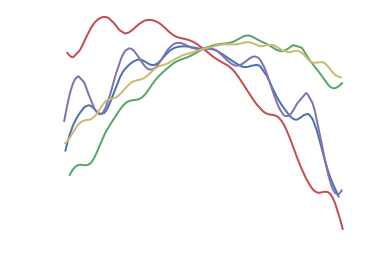
\includegraphics[width=.1\textwidth]{figs/gpSamples/main.png}
\\
SE $\times$ LIN $+$ PER $\times$ LIN $+$  RQ $\times$ LIN}
      child{ node [  align=center]{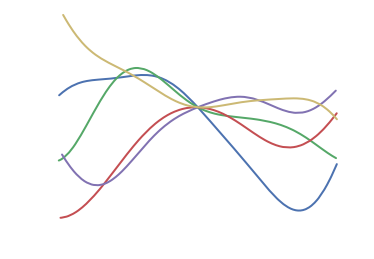
\includegraphics[width=.1\textwidth]{figs/gpSamples/selin.png}\\ SE $\times$ LIN} 
	      child{ node [   align=center] {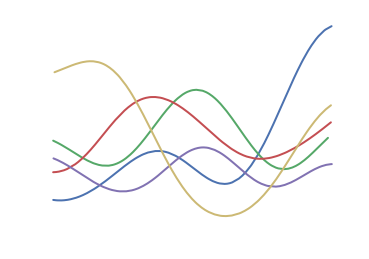
\includegraphics[width=.1\textwidth]{figs/gpSamples/se.png}\\ SE}}
	      child{ node [   align=center] {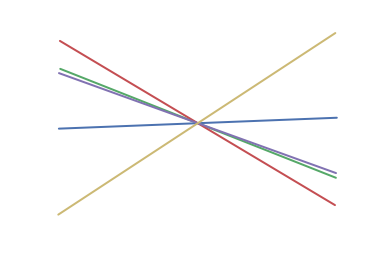
\includegraphics[width=.1\textwidth]{figs/gpSamples/lin.png}\\ LIN }}                            
      }
        child{ node [  align=center]{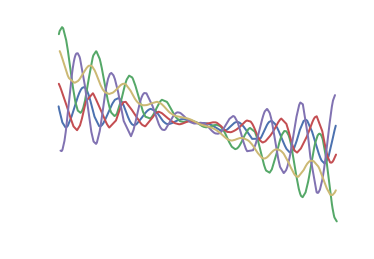
\includegraphics[width=.1\textwidth]{figs/gpSamples/perlin.png}\\ PER $\times$ LIN} 
            child{ node [   align=center] {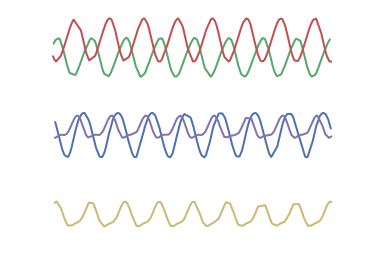
\includegraphics[width=.1\textwidth]{figs/gpSamples/per.png}\\ PER}} 
            child{ node [   align=center] {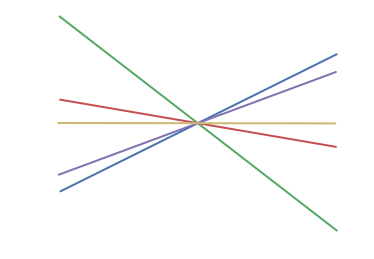
\includegraphics[width=.1\textwidth]{figs/gpSamples/lin2.png}\\ LIN}}
		}
      child{ node [  align=center]{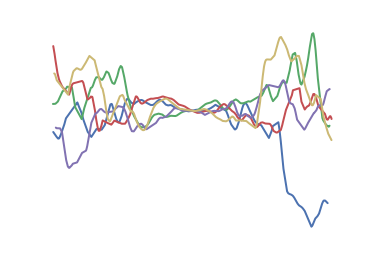
\includegraphics[width=.1\textwidth]{figs/gpSamples/rqlin.png}\\ RQ $\times$ LIN} 
            child{ node [   align=center] {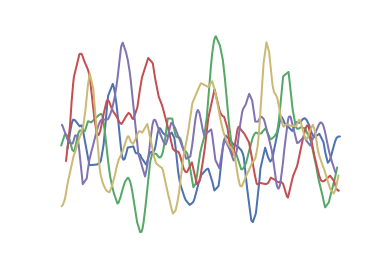
\includegraphics[width=.1\textwidth]{figs/gpSamples/rq.png}\\ RQ}}
            child{ node [   align=center] {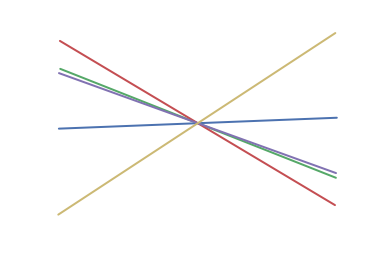
\includegraphics[width=.1\textwidth]{figs/gpSamples/lin.png}\\ LIN}}
		}
; 
\end{tikzpicture}
